\subsection{Simulation}

The software simulation is intended to design, test and simulate a possible implementation of the \ac{isa} on the level of individual logic gates. It allows an estimation of the size, complexity and number of components of its hardware equivalent. It also offers low cost and high speed of iteration. If a graphical tool is used, it also provides an opportunity visualize the entire structure. For this work, the digital logic simulator ``Digital'' by Heinz Neemann is used \cite{neemann_digital}. It is free to use and well documented and was previously used by the author to simulate other logical circuits. For these reasons, the cost of entry in both money and time spent learning to use the tool are minimal. The tool simulates digital logic circuits, which can then be hierarchically combined to form more and more complex circuits. \autoref{fig:digital_full_adder} shows a circuit that implements a 1 bit full adder within the software. \autoref{fig:digital_full_adder_reuse} shows how this circuit can then be reused in higher-level circuits.

\begin{figure}[h!]
    \centering
    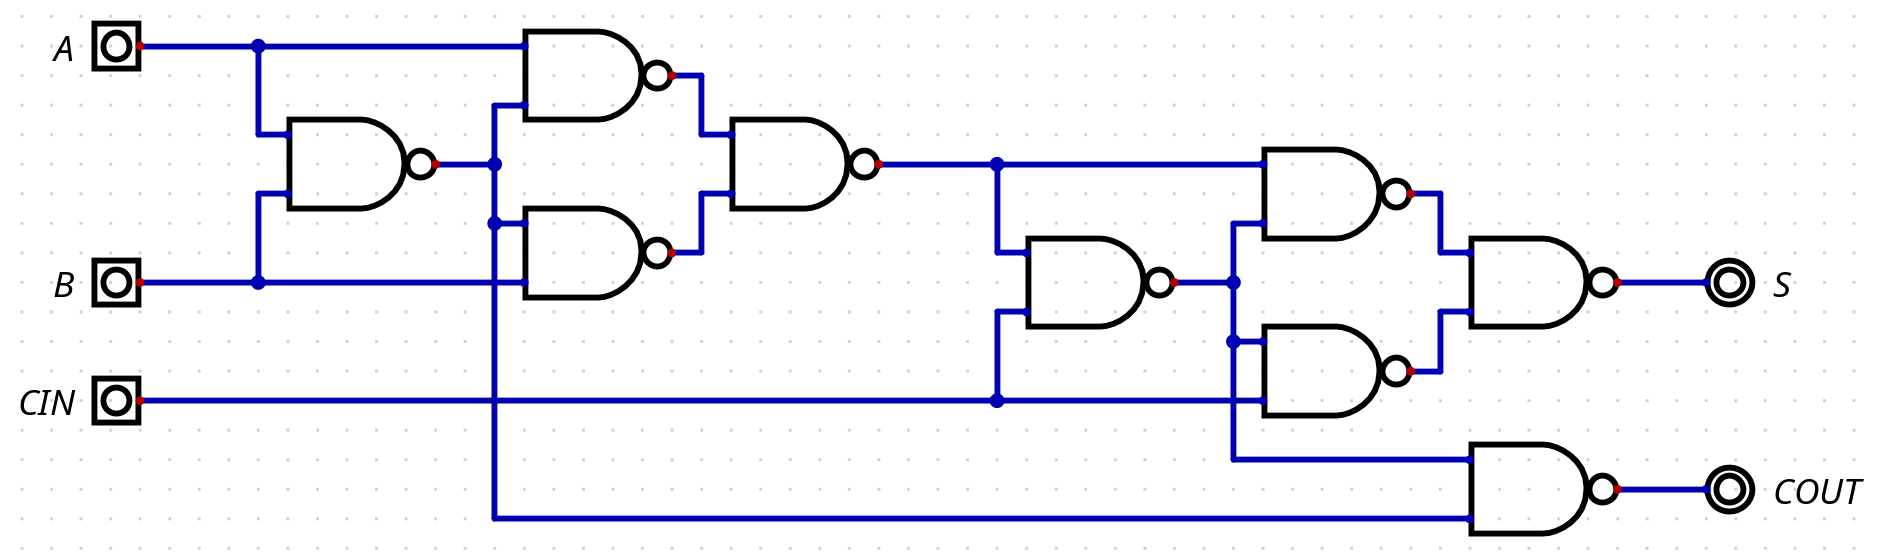
\includegraphics[width=0.8\textwidth]{images/digital_full_adder.png}
    \caption{1 Bit full adder in the logic gate simulator ``Digital''}
    \label{fig:digital_full_adder}
\end{figure}

\begin{figure}[h!]
    \centering
    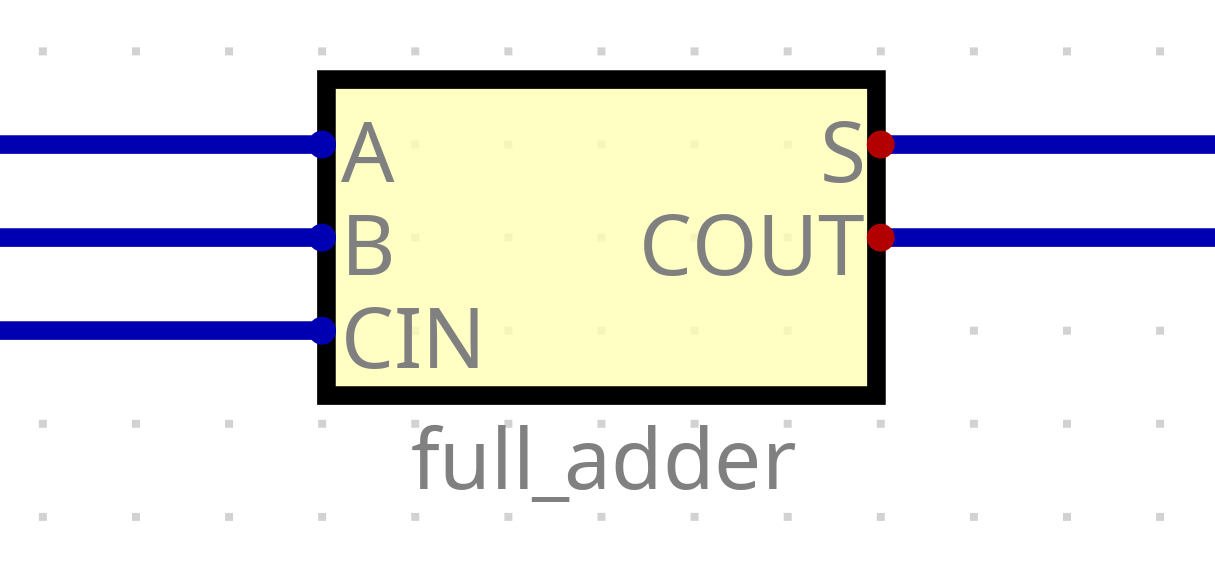
\includegraphics[width=0.8\textwidth]{images/digital_full_adder_reuse.png}
    \caption{Hierarchical reuse of the 1 bit full adder shown in \autoref{fig:digital_full_adder}}
    \label{fig:digital_full_adder_reuse}
\end{figure}

This hierarchical nesting of circuit implementations allows for easier management of large numbers of gates, as well as reuse of common components. For example, 8 instances of the same 1 bit full adder can be connected to form an 8 bit word full adder. This approach of nesting also naturally leads to better semantic grouping of circuits, which can later be reused to divide the hardware implementation into reasonably sized \acp{pcb}. The entire simulation is built from the bottom up, i.e modules that require no submodules internally and consist only of atomic logic gates are designed first. In this work, the register is the initial module to be implemented. In \autoref{sec:design_philosophy}, the requirement of using only \texttt{NAND} gates is given. Therefore, the atomic building block within the simulation is an individual 2-input \texttt{NAND} gate.

From this type of gate, the individual modules described in \autoref{sec:implementation_logical} are built. However, the diagram developed in this chapter did not yet contain any clock signals, as they are not relevant to the datapaths. However, to simulate a logic circuit, it must have a clock input. Therefore, an additional module is introduced, which is only necessary for the simulation. 

\subsubsection{Register \& Register File} \label{sec:implementation_software_simulation_register}

The register consists fundamentally of a bistable configuration of logic gates, such as latches as discussed in \autoref{sec:fundamentals_timing_sequential}. By extending an SR-latch with two more \texttt{NAND} gates, a ``gated D latch'' is created. It has two inputs $D$ and $E$, which serve as the data to store and the enable signal, respectively. When the signal $E$ is \texttt{HIGH}, the SR-latch stores the value of $D$ at that time. When $E$ is \texttt{LOW}, the state remains unchanged. \autoref{fig:implementation_software_simulation_d_latch} shows such a gated D latch implemented using only \texttt{NAND} gates.

\begin{figure}[H]
    \centering
    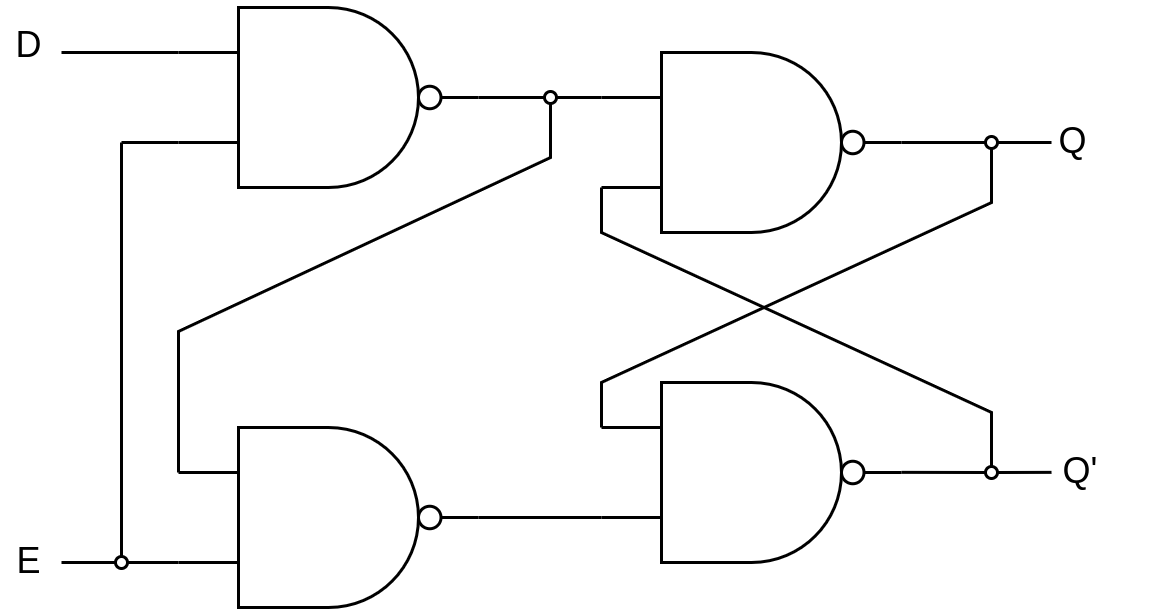
\includegraphics[width=0.7\textwidth]{images/drawio/nand_d_latch.png}
    \caption{D Latch implemented using only NAND gates}
    \label{fig:implementation_software_simulation_d_latch}
\end{figure}

However, this is not suitable for use in synchronous circuits, since the state of the latch can change multiple times when the enable signal is \texttt{HIGH}. For this reason, two such latches are combined as shown in \autoref{fig:implementation_software_simulation_clocked_d_latch}. In this configuration, the output $Q$ of the first latch is used as the input $D$ of the second one. The enable signals are shared, with one latch receiving the inverse of the other. This way, an edge detection is implemented. The new value $D$ is only propagated when the state of the clock signal changes. This circuit is suitable for synchronous circuits since the saved value can only change once at the time of a clock edge.

\begin{figure}[H]
    \centering
    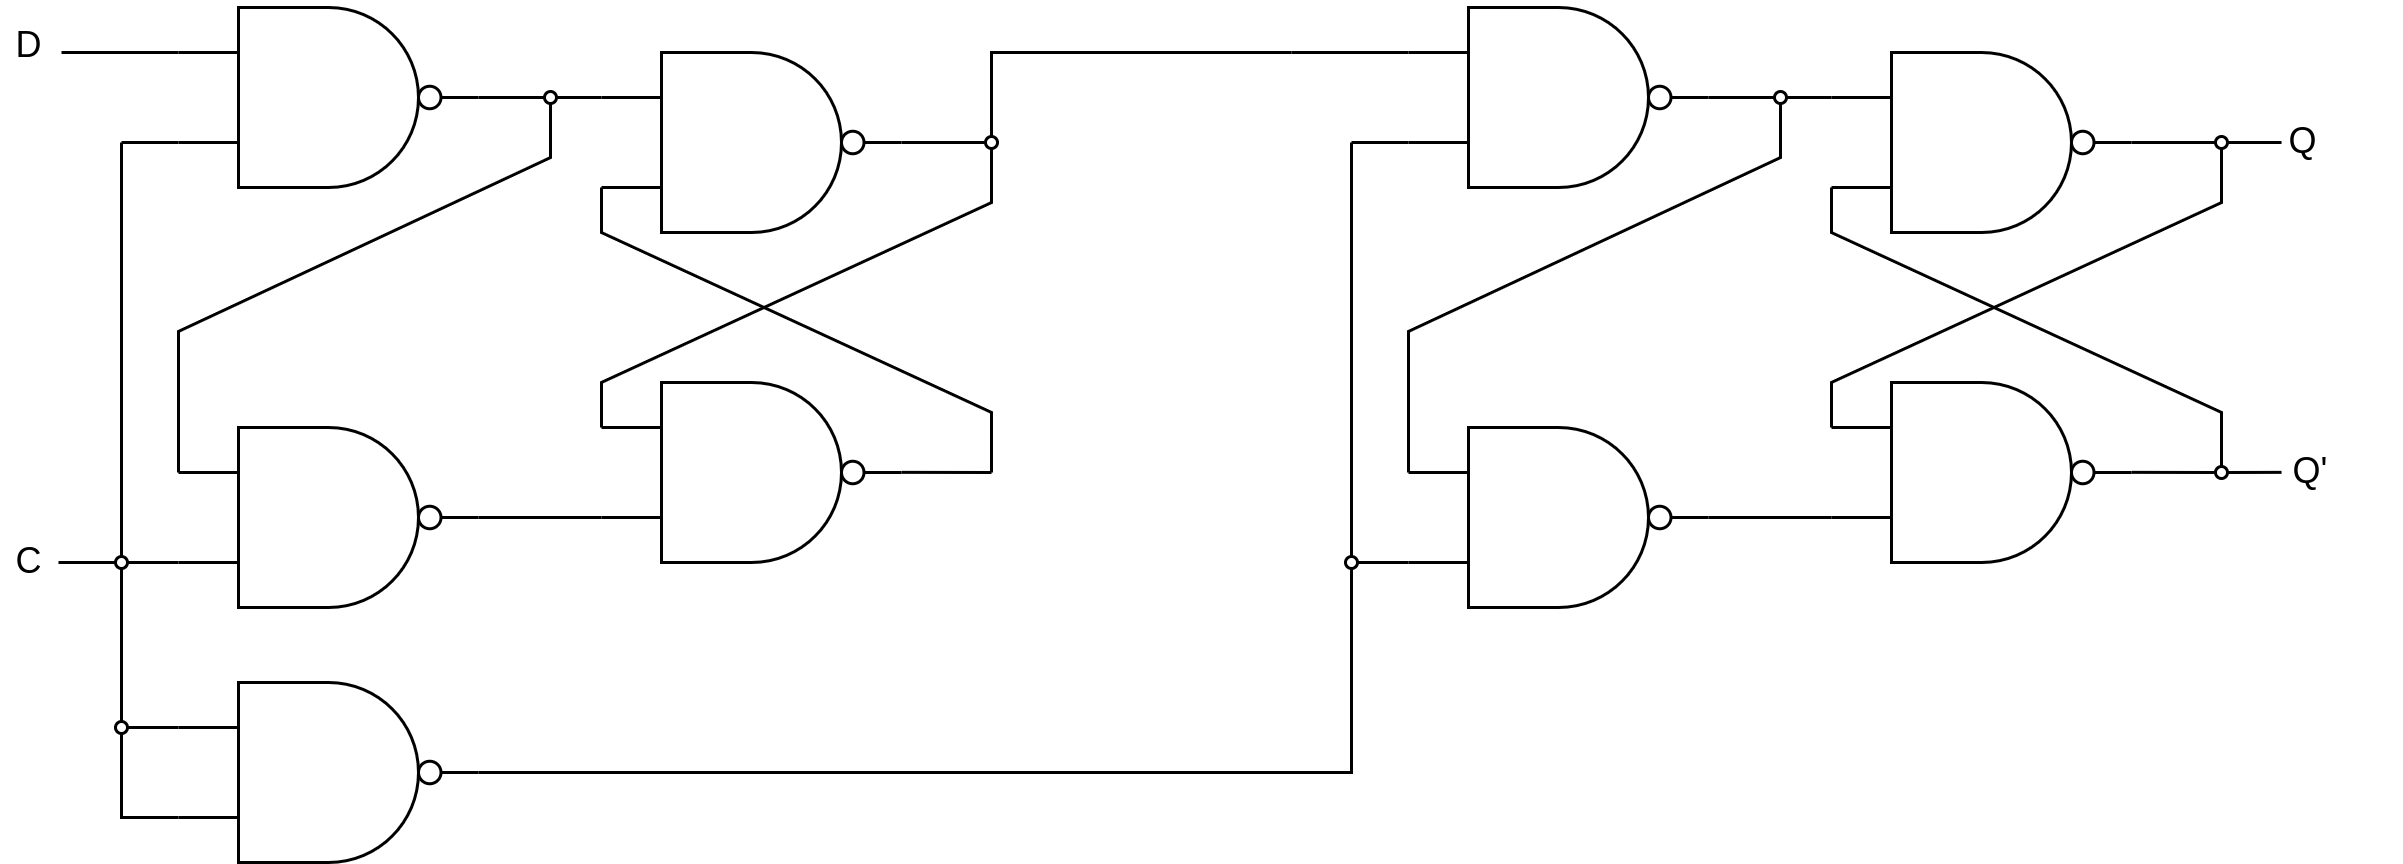
\includegraphics[width=0.9\textwidth]{images/drawio/nand_clocked_d_latch.png}
    \caption{Two sequential D latches, forming a gated, clocked D latch}
    \label{fig:implementation_software_simulation_clocked_d_latch}
\end{figure}

Eight of these gated, clocked D latches are combined in parallel to form an 8 bit register. The register has additional logic to implement its control inputs for clearing and enabling or disabling writing on each clock cycle. Multiple of these register modules are combined to form both the register file and program counter.

\subsubsection{Multiplexer}

The multiplexer is another essential low level building block that is used at several places in the logical design. It also requires no submodules internally and is built using only \texttt{NAND} gates. Due to its simple, repetetive construction, as is explained in \autoref{sec:implementation_modularisation_multiplexer}, the reconstruction in the simulation environment is not explored in more detail. The final software simulation uses several 8 bit 2:1 and 16 bit 2:1 multiplexers to select between 8 or 16 bit words, as well as a few 1 bit 2:1 multiplexers for switching control signals.

\subsubsection{Memory}

While memory can also be constructed from individual logic gates, most real working memories at the time of writing work based on electrophysical principles such as capacitance. The simulation software that is used in this work does not capture such analog quantities. Additionally, as seen in \autoref{sec:implementation_software_simulation_register}, storing even a single bit requires multiple logic gates. Therefore, creating any significant amount of memory from discrete logic gates is not feasible, especially since the address space of the AVA \ac{isa} spans 65536 bytes or 524288 bits of memory. Furthermore, the computational overhead for the simulation software would be substantial for something not directly relevant to the computation performed by the device. For these reasons, memory is provided as its own building block. For these reasons, the memories, including working \ac{ram} and program and instruction \ac{rom} are the the only building blocks that do not internally consist of simulated \texttt{NAND} gates. The simulation software can be configured to load the contents of program and control signal \ac{rom} on each start of the simulation. Working memory is initialised to contain only the value 0.

\subsubsection{Clock \& Interface unit}

The clock \& interface unit provides a way to interact with the state of the simulated device. It has inputs in the form of a clock generator and several buttons controlling the following aspects:

\begin{description}
    \item[Reset] Clears all registers
    \item[Halt] Manually halts the device, stopping clock propagation
    \item[Continue] Manually resumes operation if the device is halted
    \item[Step] Manually execute one phase of the instruction cycle
    \item[Clken] Enable or disable clock signal generation     
\end{description}

Since this unit is only relevant for the software simulation, it is not explained in more detail.

\subsubsection{Arithmetic logic unit}

The \ac{alu} is fully asynchronous, and as such can be implemented using only \texttt{NAND} gates. Due to the inherent complexity and number of gates, it is internally further subdivided into three functional modules:

\begin{itemize}
    \item Addition \& Subtraction
    \item Boolean logic
    \item Bit-shifting
\end{itemize}

Each of these modules implements one class of arithmetic or logical operators. Their outputs are combined using multiplexers, which are controlled using the \ac{alu} opcodes. Similarly, since the output of the set of flags also depends on the operation, more multiplexers are used to select the source of the corresponding flag.

Addition is implemented using an 8 bit ripple-carry adder. It consists of 8 full adders, each of which receives the carry input of the previous unit, except for the first one, which receives the carry flag of the last operation. While this is relatively slow, improvements such as carry-lookahead adders are more complicated to implement and do not visualize the operation as clearly. \autoref{fig:implementation_software_simulation_full_adder} shows a single full adder built using only \texttt{NAND} gates. Its two outputs compute by the following boolean expressions:

\begin{align}
    S &= A \lxor B \lxor CIN \\
    COUT &= (A \land B) \lor (CIN \land (A \lxor B))
\end{align}

\begin{figure}[H]
    \centering
    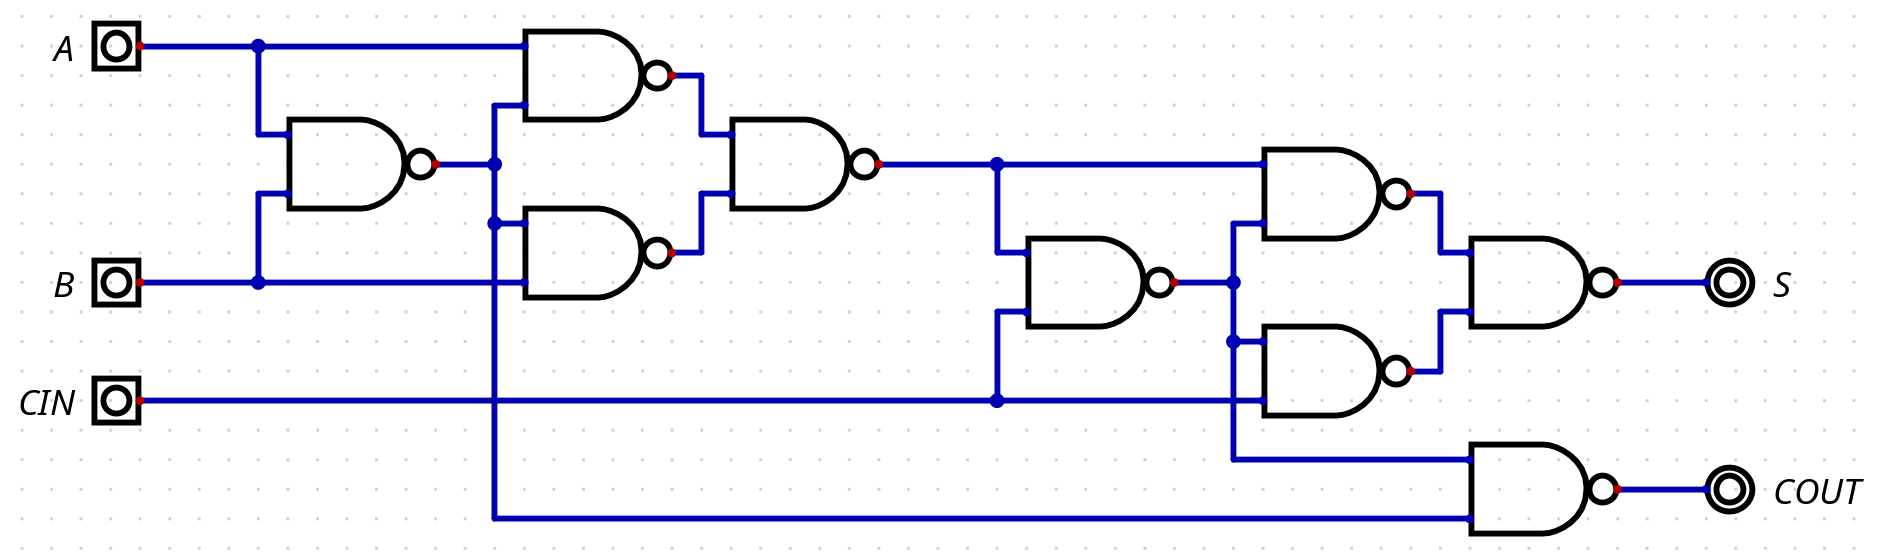
\includegraphics[width=0.9\textwidth]{images/digital_full_adder.png}
    \caption{Full adder implemented using only \texttt{NAND} gates}
    \label{fig:implementation_software_simulation_full_adder}
\end{figure}

\begin{wrapfigure}{R}{0.5\textwidth}
    \centering
    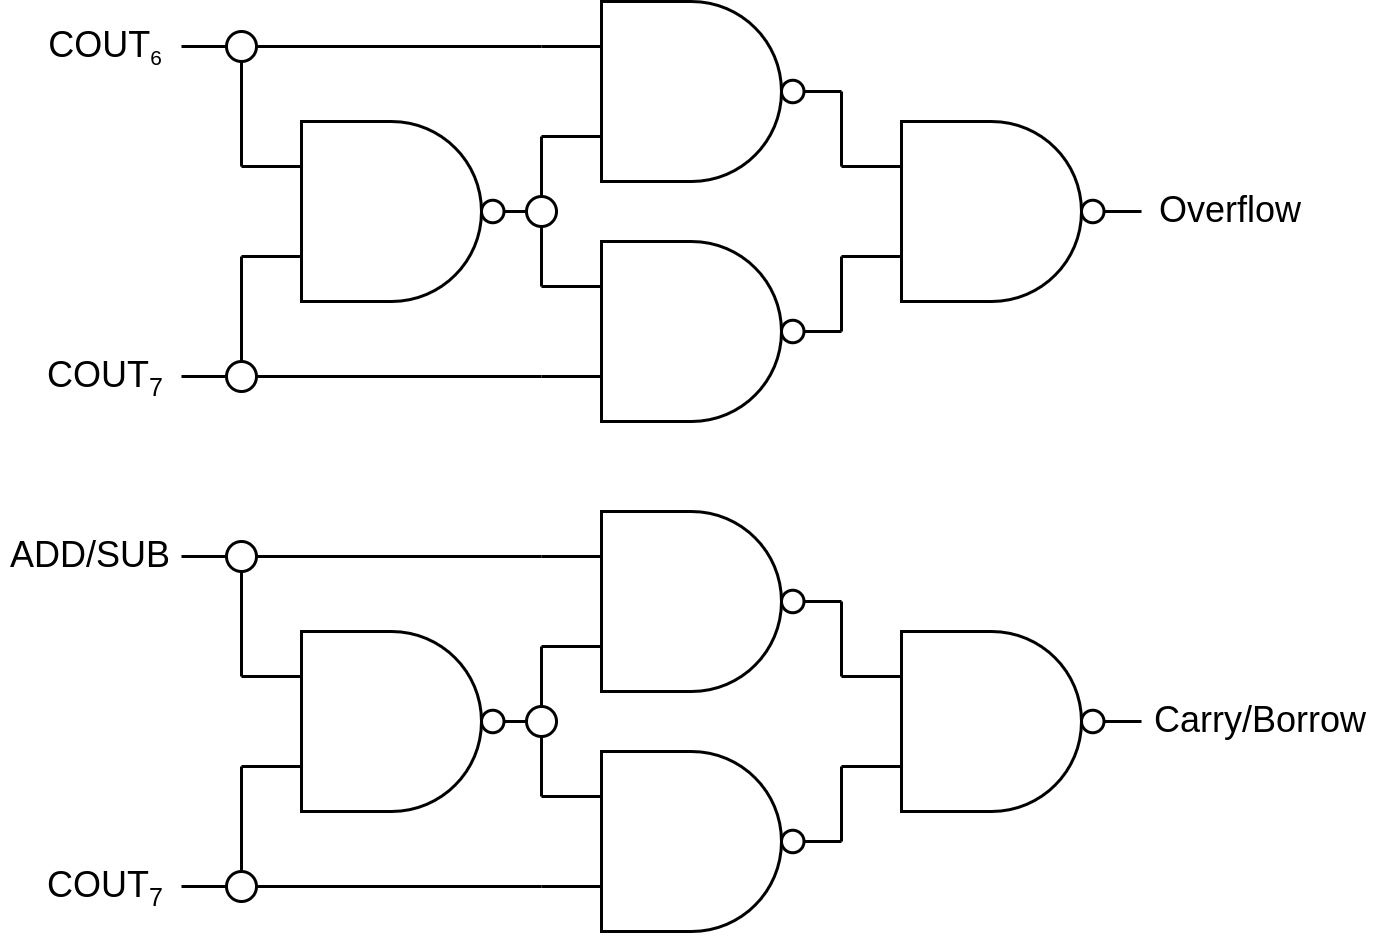
\includegraphics[width=0.48\textwidth]{images/drawio/addsub_overflow_carry.png}
    \caption{Logic gate circuits that compute carry/borrow and overflow flags for addition and subtraction}
    \label{fig:implementation_software_simulation_addsub_overflow_carry}
\end{wrapfigure}\leavevmode

Due to the two's complement representation of negative numbers, subtraction is implemented by inverting all bits of the second operand and adding the value 1. By using the carry input of the adder circuit, this constant can be added implicity. Inversion is implemented by using the \texttt{XOR} logic gate with the constant 1 at one input. Since this module receives only one bit of the \ac{alu} opcode to distinguish between addition and subtraction, this bit can be used instead of the constant 1. Both addition and subtraction output their carry-out, as well as the overflow flag as defined in the \ac{isa}. An overflow occurs when the most significant bit of the result is not enough to capture the result value. To detect this, one can simply check if the carry outputs of the last and second-to-last adder stages are different using a single \texttt{XOR} logic gate. Similarly, by combining the bit that switches between addition and subtraction and the carry output of the last adder stage, one can obtain the carry-out and borrow flag for both addition and subtraction \cite{idallen_overflow}. \autoref{fig:implementation_software_simulation_addsub_overflow_carry} shows these circuits implemented using only \texttt{NAND} gates.

\begin{wrapfigure}{R}{0.5\textwidth}
    \centering
    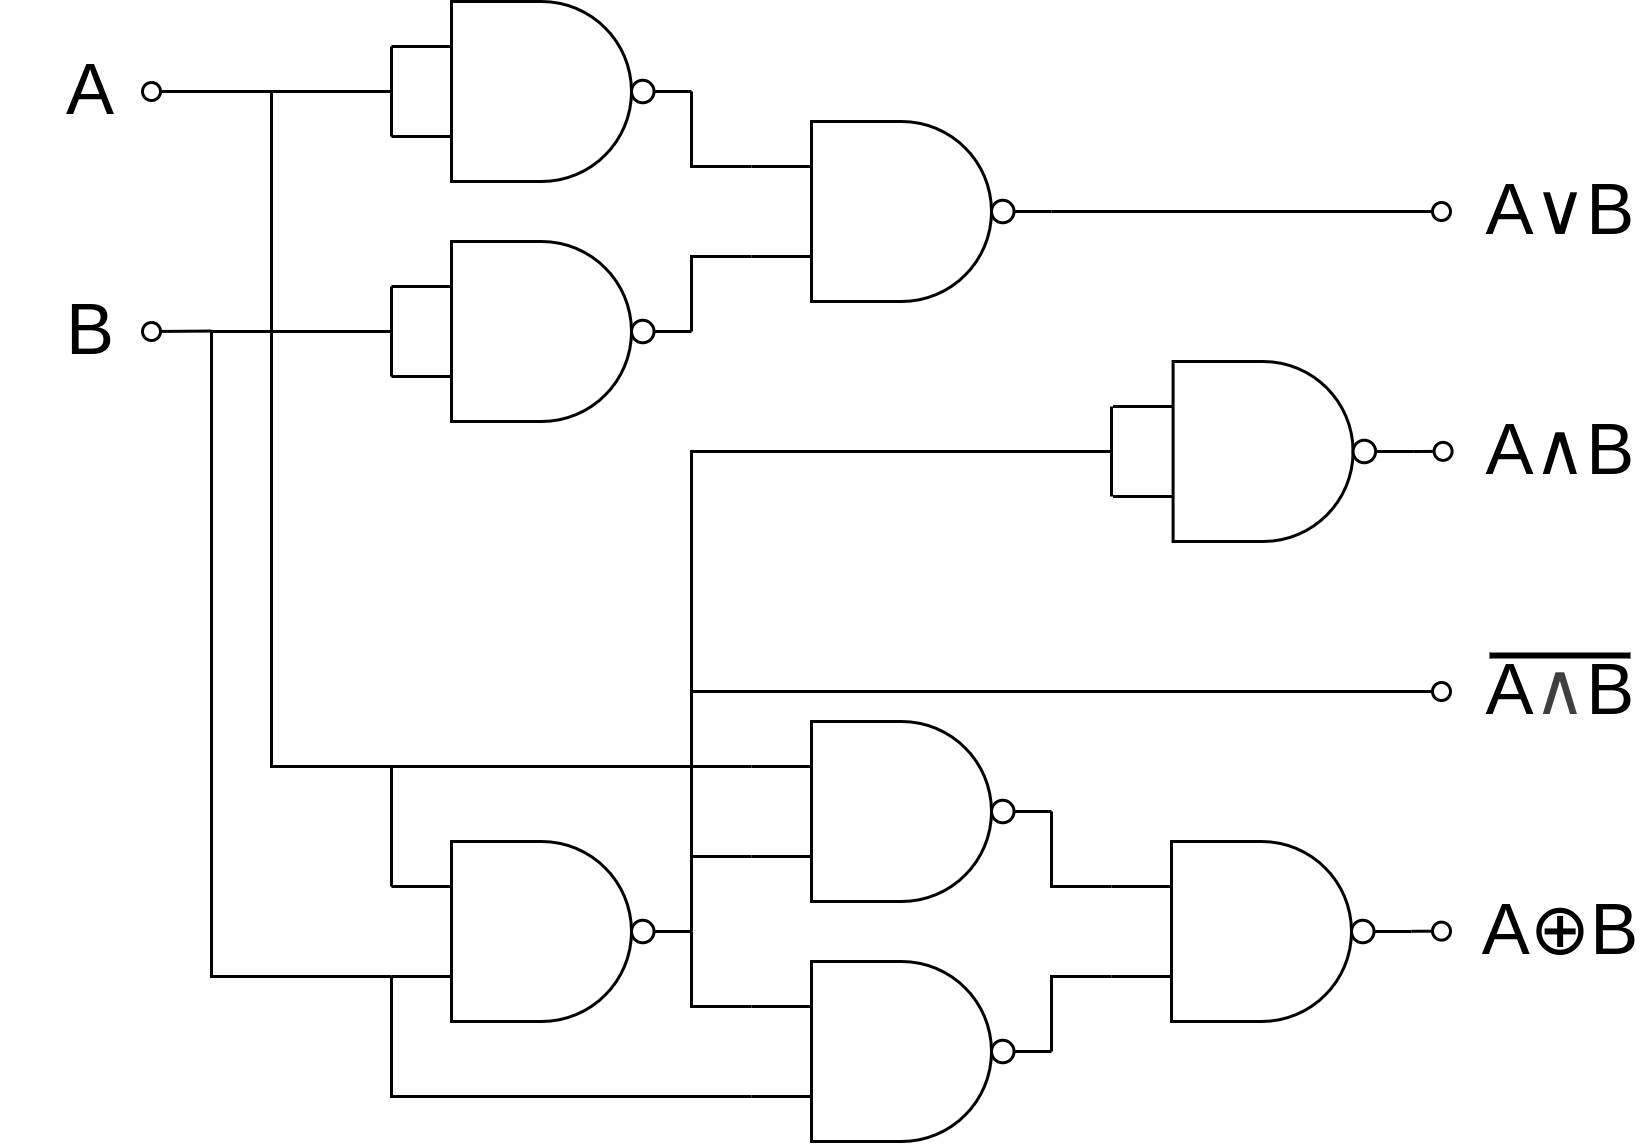
\includegraphics[width=0.48\textwidth]{images/drawio/bitwise_operators_logic.png}
    \caption{Implementation of OR, AND, XOR, NAND operators using only NAND gates}
    \label{fig:implementation_software_simulation__binary_operators}
\end{wrapfigure}\leavevmode

As discussed in \autoref{sec:implementation_opcodes}, the boolean logic module implements the four operators \texttt{\{OR, AND, XOR, NAND\}}. \autoref{fig:implementation_software_simulation__binary_operators} shows the implementation using only \texttt{NAND} gates, as also explained in the same chapter. The boolean logic module outputs no flags.

The bit shifting module is implemented using a series of 8 bit 2:1 multiplexers. A multiplexer at stage $n$ either passes the output of stage $n - 1$ without change, or shifts it by $2^n$ bits by offsetting inputs and outputs by $n$ places. For 8 bit operands, all shifts by more than 7 bits result in the same value, as all 8 bits of the first operand have been replaced. Therefore, only $log_2(8) = 3$ multiplexers are required. Depending on the least significant bits of the second operand, they shift the first operand by 1, 2 or 4 bits, respectively. However, this approach has the disadvantage of requiring a separate series of three multiplexers for shifting to the left or to the right. An advantage, however, is that the inputs that are not assigned an output from the previous stage can use the value of the carry bit of the flags register to replace shifted bits by either a 0 or a 1. The boolean logic module outputs only a carry out flag, which is the first bit that was shifted out of the input. By combining this with replacing shifted bits by the last carry, data of arbitrary size can be shifted by repeatedly shifting 8 bit data in sequence. \autoref{fig:implementation_software_simulation_shifter} shows the full bidirectional shifter with all mentioned features, as it is implemented at the time of writing.

\begin{figure}[H]
    \centering
    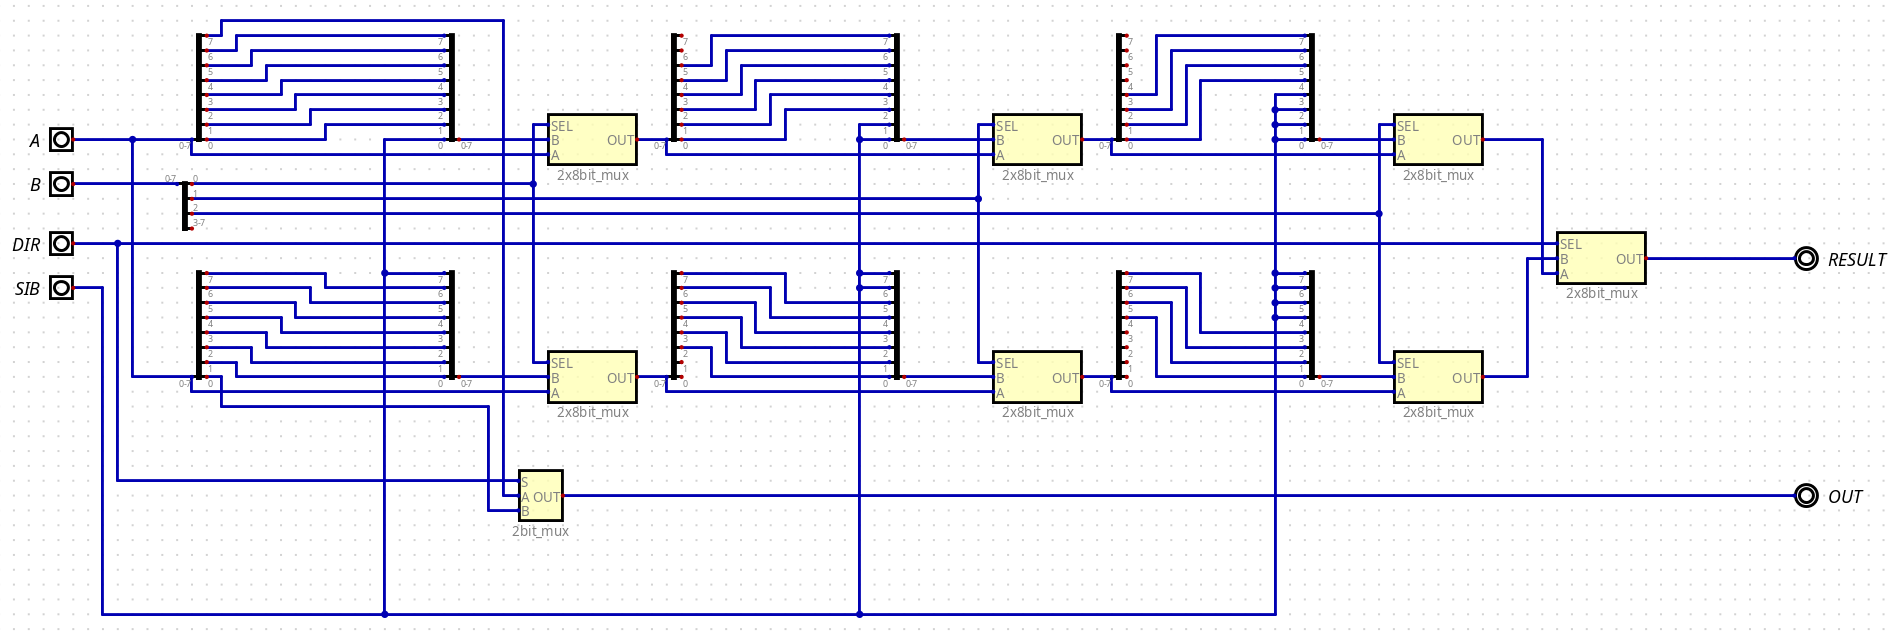
\includegraphics[width=\textwidth]{images/bitshifter.png}
    \caption{Bidirectional shifter implemented in simulation software ``Digital''}
    \label{fig:implementation_software_simulation_shifter}
\end{figure}